\subsection{Rendering}
\paragraph{}
Rendering the scene into a perceivable image is one of the core jobs of the application.
Realizing effects that approximate both real movie footage and the wishes of the user is often hard, or even impossible.
The implementation is closely tied to the abilities requested from the tool, many effects such as lighting or arbitrary depth ordering requires low level trickery with the chosen framework.

In addition, the scene does not only have to be rendered once but often twice.
Binocular vision infers depth relationships from slight differences in images taken from two separate viewpoints.

Section \ref{FrameworkOpenGL} discusses the choice of drawing framework.
Section \ref{RendCamera} discusses how a 3D scene gets mapped into a 2D image.
Section \ref{RendStereo} discusses stereo rendering methods.
Section \ref{ImplContainer} discusses the implementation of other effects.
For a high level description of many features see section \ref{sceneRep} on scene representation and \ref{Cues} on the topic of depth cues.


\subsubsection{Camera\label{RendCamera}}

\begin{figure*}[hbt]
\begin{center}
\subfigure[Perspective Cameras]{\label{CamPer}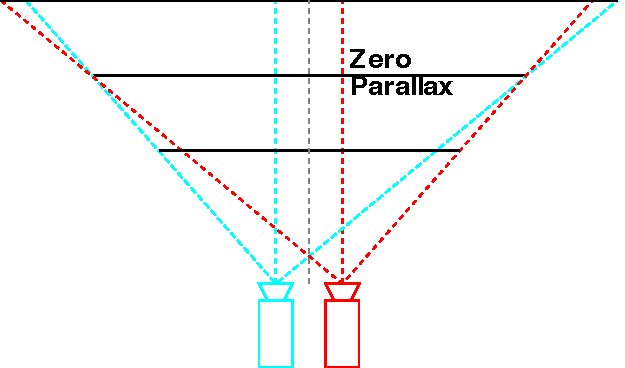
\includegraphics[scale=0.75]{media/camera-perspective.pdf}}
\subfigure[Parallel Cameras]{\label{CamPar}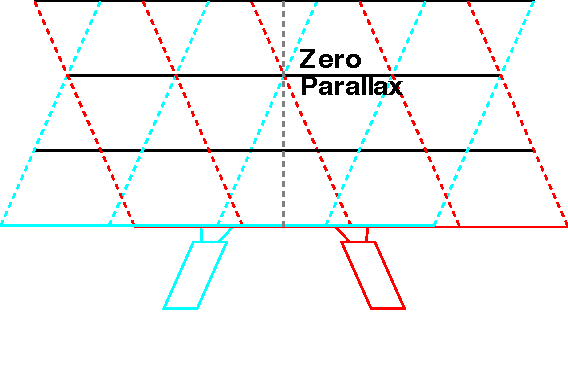
\includegraphics[scale=0.75]{media/camera-parallel.pdf}}
\caption{A diagram of the two main camera types}
\end{center}
\end{figure*}

\paragraph{}
To transform a 3D scene into a 2D picture on screen it is projected with a linear transformation.
The solution \textit{OpenGL} has is described below.
Real cameras often have non-linearities which can not be simulated with such a simplification.

To reproduce stereoscopically viewable content, two cameras are uses, representing the left and right eye.
There are several ways to place the camera and parametrize the camera, two of which are implemented in \ER\ and described below.

\paragraph{OpenGL}
In \textit{OpenGL}, the projection matrix, a 4x4 matrix, defines the projection transformation.
This is the \textit{OpenGL} equivalent of a camera.
The projection matrix depends exclusively on the type of the camera.
The position and the direction of the camera is part of the modelview matrix.

Defining such a matrix is done with convenience functions for commonly used projections or by setting up the view frustum manually.

\paragraph{Perspective Cameras}
When working with physical cameras to create stereoscopic content, the main choice is wether to place the cameras parallel or converge them.

Converging helps with establishing the zero parallax plane, but causes problems with the separation of objects behind and in front of it.

Parallel cameras limit the divergence to the camera separation at the center of the image.
\ER\ uses parallel cameras.
With hardware parallel cameras, the zero parallax plane is set by shifting and cropping the two resulting images.
This is not needed in digital imaging, instead the projection matrix is adjusted to an asymetric frustum.
Figure \ref{CamPer} shows a schematic of this setup.

\paragraph{Parallel Cameras}
Parallel projecting cameras are not used in hardware.
They have some interesting properties that make them desirable in testing stereoscopic effects,
namely their elimination of relative size, motion and other perspective clues.

To get stereoscopic images that can be fused, converged cameras have to be used.
In \ER\ the camera projection matrix is skewed so that the projection planes of left and right camera are parallel, and the projection direction is non-perpendicular to it.
Figure \ref{CamPar} shows this setup.


\subsubsection{Stereo\label{RendStereo}}
\paragraph{}
Ideally, the output of the program is either intended to be viewed without binocular vision, or a projector solution is used.
Then the scene is simply rendered twice into different windows or in split screen.
If the used graphic hardware supports it, \textit{OpenGL}'s QuadBuffering can be used to easily drive many types of stereoscopic viewing systems.

\paragraph{Anaglyph}
For a quick and easy preview on any screen, anaglyph is the simplest method.
Many different variations of anaglyph are used, the most popular of which are red-blue and red-green coding.
A simple implementation based could draw only the red channel of the image intended for the left eye, and the green and blue channel of the right eye.
Unfortunately this leads to rivalry when rendering scenes that contain objects that consist mostly of those colors.

The correct way is to mix all colors of one side into it's channel.
The loss of color contrast is made up with the better fuseability and the reduction in rivalry.

\todo{Write about rendering for stereoscopic vision, such as Anaglyph/SidebySide}

